% !TeX root = ../../Thesis.tex
\chapter{Effects of laser bandwidth on inflationary stimulated Raman scattering}
\label{chp:broadbandSRS}

In this chapter, results of one-dimensional PIC simulations are presented, which represent the first investigation into the practical possibility of using broadband to suppress inflationary SRS in shock-ignition. The chapter begins with a review of the literature discussing suppression of SRS by broadband lasers. We then show that for a decoupled broadband laser, the non-linear frequency shift must be taken into account when calculating the condition for suppression of iSRS. Next we consider the case of realistic shock-ignition schemes on three laser systems: frequency-tripled ND : glass; Krypton Fluoride (KrF); and Argon Fluoride (ArF). In each of these cases we model the predicted maximum realistic bandwidth in its physically-correct functional form. The chapter concludes with a discussion of the limitations of the modelling done so far, and suggestions for future work.

\section{Motivation and literature review}

Early results in the 1970s suggested that finite-bandwidth laser drivers could change the behaviour of parametric instabilities. These studies considered a variety of parametric instabilities, including: the parametric decay instability \citep{Thomson1974}; stimulated Brillouin scattering \citep{Kruer1973}; and stimulated Raman scattering \citep{raymer_theory_1979}. Recently, broadband has become a fashionable topic of discussion. There are various ways that broadband can be introduced into a laser system, including: induced spatial incoherence (\acrshort{ISI}) \citep{Lehmberg198327}; smoothing by spectral dispersion (\acrshort{SSD}) \citep{Skupsky1989}; stimulated rotational Raman scattering (SRRS);  In what follows, we divide the literature review by the type of SRS considered: absolute; convective-fluid; and inflationary. The effects of different forms of bandwidth are discussed within these subheadings.

\subsection{Absolute SRS}
In the case of absolute SRS in inhomogeneous plasma, the absolute instability threshold can be increased by using bandwidth.

Studies have also been performed using the code LPSE which show that, at ignition scales, absolute multi-beam backward SRS can be mitigated with bandwith $\sim 1.6\%$ \citep{Follett2021}.

\subsection{Fluid convective SRS}
These anlytical results are based on random
Bandwidth weakens coupling but increases the length of the resonance region, cancelling out when laser bandwidth greater than homogeneous growth rate \citep{Guzdar1991}.

\subsection{Inflationary SRS}
\citet{Wen2021} derive a condition for the maximum gain of SRS driven by a sinusoidally frequency-modulated broadband laser, when the velocity of the resonance point is equal to the group velocity of the back-scattered light for as long as possible. By tuning the plasma parameters and/or laser parameters away from this condition, they can increase the threshold for kinetic SRS \citep{Wen2021}. The maximum gain criteria is given by the expression:

\begin{equation}\label{eqn:maxGainCondition}
 \Delta\omega\omega_m = \omega_{pe}c / 2L_n,
\end{equation} and is verified through PIC simulations in the kinetic and fluid regimes. The left-hand side of Eq. \ref{eqn:maxGainCondition} represents the maximum chirp ($|\partial_t\omega_0(x,t)|$) of the laser, and the right-hand side gives an expression for the spatial detuning due to density inhomogeneity. Several simplifying assumptions are made by the authors which allow them to derive this expression for the spatial detuning. Most importantly for our work, they omit the contribution of the non-linear frequency shift in their calculation of the velocity of the resonance point. \todo{Estimate size of this contribution in my cases and hope it is ignorable}

A key result of this work is that the threshold for iSRS driven by a sinusoidally frequency-modulated laser is independent of the bandwidth or frequency modulation alone, rather it depends on their product. Figure \ref{fig:Wenreplication} shows results from our benchmarking of Wen's work. In this benchmarking study we recovered the results of their Osiris study using our own PIC code, EPOCH. We ran several simulations with fixed maximum normalised chirp ($\Delta\omega \omega_m / \omega_0=5.5\times10^{-6}$) and varied bandwidth. We find that the inflation threshold has a weak dependence on the bandwith alone. From this preliminary investigation, we were confident in our laser set-up and in the use of EPOCH for this project.


\begin{figure}[ht]
   \centering
    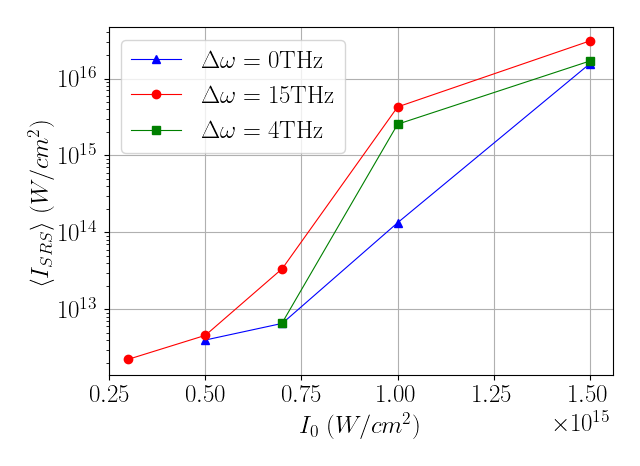
\includegraphics[width=0.75\columnwidth]{Chapters/C5_broadband/bandwidth_no_dependence_Wen.png}
    \caption{Intensity of light scattered by SRS, averaged over the last three picoseconds of each simulation, for three laser set-ups with fixed maximum normalised chirp ($\Delta\omega \omega_m / \omega_0=5.5\times10^{-6}$) and varied bandwidth. The simulation parameters common to all data-points are: $T_e = 4\si{\kilo eV}; L_n = 400\si{\micro\metre}; n_e(x) = 0.11n_{\text{cr}}; \text{exp}(x/L_n);\text{PPC=16,000}. $}
    \label{fig:Wenreplication}
\end{figure}{}


\section{Decoupled broadband lasers}

The work in this section was presented at the 62nd annual meeting of the American Physical Society Division of Plasma Physics in November 2020.
 
The first approach we considered was using a decoupled broadband laser, as presented by Zhao. 

In \cite{zhao_suppression_2019} they consider the suppression of parametric
instabilities in a homogeneous plasma by decoupled broadband lasers
(\acrshort{DBL}). A
decoupled broadband laser is defined in Ref \cite{zhao_effective_2017} as

\begin{equation}\label{eqn:DBL}
  a_{\mathrm{DBL}} = \sum_{i=1}^{N} a_i \mathrm{cos}(\omega_it + \phi_i),
\end{equation}
where $a_i,\omega_i,\phi_i$ are the amplitude, carrier frequency, and phase of
each of the $N$ beamlets. The central frequency and wavelength of the laser is
$(\omega_0,k_0)$ and the total frequency spectrum bandwidth is
$\Delta\omega_0$.
Considering the frequency difference between any two beamlets, they find that
there is a critical frequency difference below which the SRS instability regions
for the beamlets overlap to form a single instability region. In this case, the
two beamlets can be coupled with one EPW, leading to a higher growth rate for
SRS. An important result of their one-dimensional PIC simulations is that iSRS
instability can grow to a high level if the beamlets satifsy this coupling
condition, even if the total bandwidth is very large.


In Ref \cite{zhou_kinetic_2018} Zhou \textit{et al.} consider the case of SRS
driven by a broadband laser for a homogeneous plasma, with NIF-relevant plasma
density and temperature such that $\kld > 0.3$. The result most relevant to our
work is that the bandwidth can interact with the nonlinear frequency shift associated
with electron trapping in the SRS EPW to \emph{enhance} SRS rather than suppress it.



Zhao \textit{et al.} \cite{zhao_effective_2017} consider the case of an
inhomgeneous plasma density profile relevant to indirect-drive ICF. The results
are similar to those described in the homogeneous case, and they find a
condition for the complete suppression of SRS. The follow-up paper
\cite{zhao_suppression_2019} finds that SRS can be well controlled for a laser
beam structure of multiple frequency components and total bandwidth of a few
percent. The parameters considered in this study are
$\lambda_0=0.33\si{\micro\metre}$,
$T_e=2\si{\kilo\electronvolt}$, $n_e = [0.08,0.12]n_c$, giving $\kld \sim
[0.26,0.35]$, well within the kinetic regime for SRS.

They derive a gain exponent for standard convective SRS driven by two
beamlets of different frequencies, and find that two beamlets are independent
when
\begin{equation}\label{DLB_threshold_inhomo}
\delta \omega_{0} \geq \frac{\pi n_{0} c\left(\omega_{0}^{2}-\omega_{p
e}^{2}\right)^{3 / 2}}{8 L \omega_{0} \omega_{L}^{2} \nu_{p}^{2}}.
\end{equation}
Importantly, this condition is independent of the amplitude of the incident
laser. In theory, this condition would allow us to construct a DBL to suppress
SRS in a large-scale inhomogeneous plasma, however, secondary amplification of
back-scattered light by one of the beamlets is a possibility. We must therefore
consider another threshold for this secondary amplification: $\delta\omega_0 >
\omega_{L1}-\omega_{L2}$ where $[\omega_{L1},\omega_{L2}]$ is the range of EPW
frequencies excited by SRS in the plasma (not including nonlinear frequency
shift).


\subsection{Conclusions}
In conclusion, we decided not to pursue out investigation of DBL-type bandwidth any futher since a) there are no plans to impliment it on lasers of interest and b) 


\section{Realistic laser bandwidth}\label{sec:params}

This section concerns the results of our investigation into broadband suppression of inflationary SRS on different broadband laser systems. The particular form of the broadband may not seem like an important factor to us, but to the EPWs it can be very important.
We consider shock-ignition driven by three different laser systems: frequency-tripled Nd : glass lasers, such as the NIF and LMJ; KrF lasers; and ArF lasers. Each laser has a different frequency and native bandwidth. For the so-called excimer lasers (KrF and ArF) 

For all the simulations presented in this section, the following EPOCH parameters are constant: $\Delta x = \mathrm{min}_x(\lambda_D)$; $\mathrm{PPC} = 2000$; $T_{\mathrm{end}}=6\si{ps}$; thermal boundaries for particles; field boundaries are laser ($x_{\mathrm{min}}$), and absorbing boundaries ($x_{\mathrm{max}}$). We treat the ions as a neutralising background population to allow us to pinpoint the effect of bandwidth on inflationary SRS only. The incident laser intensity is set to be approximately the threshold intensity for inflationary SRS. The threshold intensity is found by varying the intensity for identical PIC set-ups to find the minimum intensity such that the time-averaged intensity of scatter from bSRS is greater than $10\%$ of the incident laser intensity. 

\begin{table}[h]\label{tab:laser}
\begin{center}


\begin{tabular}{|l|l|l|l|}
\hline
\begin{tabular}[c]{@{}l@{}}Wavelength /\\ nm\end{tabular} & \begin{tabular}[c]{@{}l@{}}Intensity / \\ W$\text{cm}^{-2}$\end{tabular} & \begin{tabular}[c]{@{}l@{}}Bandwidth / \\ THz\end{tabular} & \begin{tabular}[c]{@{}l@{}}Bandwidth / \\ $\%$ $\omega_0$\end{tabular} \\ \hline 
&&&\\[-1em]
351   & $3\times 10^{15}$  &  0, 1, 10 &  0, 0.02, 0.20 \\ \hline
&&&\\[-1em]
248   &    & 0, 3, 6  &     \\ \hline
&&&\\[-1em]
193   & $4\times 10^{15}$   & 0, 5, 8, 10  & 0, 0.05, 0.08, 0.10  \\ \hline
\end{tabular}
\end{center}
\caption{Laser parameters for this investigation. Where multiple values are presented in a list, each represents a different simulation. The incident laser intensity is set to be approximately the threshold intensity for inflationary SRS. The choice of bandwidths and their implementations in EPOCH are explained and referenced in Sections \ref{sec:351}, \ref{sec:248}, \ref{sec:193}, for the 351, 248, 193 nm cases respectively.}
\end{table}

\begin{table}[h]
\begin{center}

\begin{tabular}{|l|l|l|l|l|l|}
\hline
Wavelength / nm & $L_x$ /$\si{\micro\metre}$ & $T_e$ / keV & $n_e$ / $n_{cr}$ & $\omega_{pe}$ / $\omega_0$ & $L_n$ / $\si{\micro\metre}$
\\ \hline 
351 & 270 & 5.4 & $[0.105,0.175]$ & $[0.33,0.42]$ &  $[420,590]$ \\ \hline
248 & ? & ? & ? & ? &  ? \\ \hline
193 & ? & ?  & ?   & ?               & ? \\ \hline

\end{tabular}

\end{center}
\caption{Table shows plasma parameters from simulations performed at the NRL, chosen such that $\kld$ is between 0.3 and 0.45. The temperature given is the maximum temperature of the particles initialised at $t=0$, as there is, in reality, a slight temperature gradient in the electron profile.}
\label{tab:plasma}
\end{table}




\section{351nm Nd : glass laser}\label{sec:351}

\subsection{Base case: $\Delta\omega=0$}
As stated in Section \ref{sec:params}, the plasma density and temperature profiles are taken from the library of radiation hydrodynamic simulations at the Naval Research Laboratory. 

\subsection{SSD-type bandwidth: $\Delta\omega=1\si{THz}$}
1THz is the maximum bandwidth currently implemented by SSD on a 351nm laser, achieved at the Omega laser facility \citep{Regan2005}. According to \citet{Wen2021}, in order to suppress iSRS with the parameters taken from our base case, we require that the modulation frequency satisfies $\omega_m \gg \omega_{pe} c / 2L_n\Delta\omega$. From the plasma parameters given in Table \ref{tab:plasma} and bandwidth of 1THz, this requirement becomes: $\omega_m \gg 800 \si{THz}$. This is problematic, since the optimal modulation frequency for SSD-type smoothing is on the order of $10 \si{GHz} = 0.001 \si{THz}$ \citep{Kelly2013}.

We can implement a continuous-bandwidth frequency-modulated laser in EPOCH using the standard EPOCH laser-driver: $E(x,t) = E_0\text{sin}\left(\omega_0 t - \phi(x,t)\right)$; with $\phi(x,t)$ given by:

\begin{equation}
	\phi(x,t) = \frac{1}{2}\frac{\Delta\omega}{\omega_m}\text{sin}	 	 \left(\omega_mt - \frac{\omega_m}{c}x\right).
\end{equation}


\subsection{Optical parametric amplification: $\Delta\omega=10\si{THz}$}

\begin{figure}[ht]
   \centering
    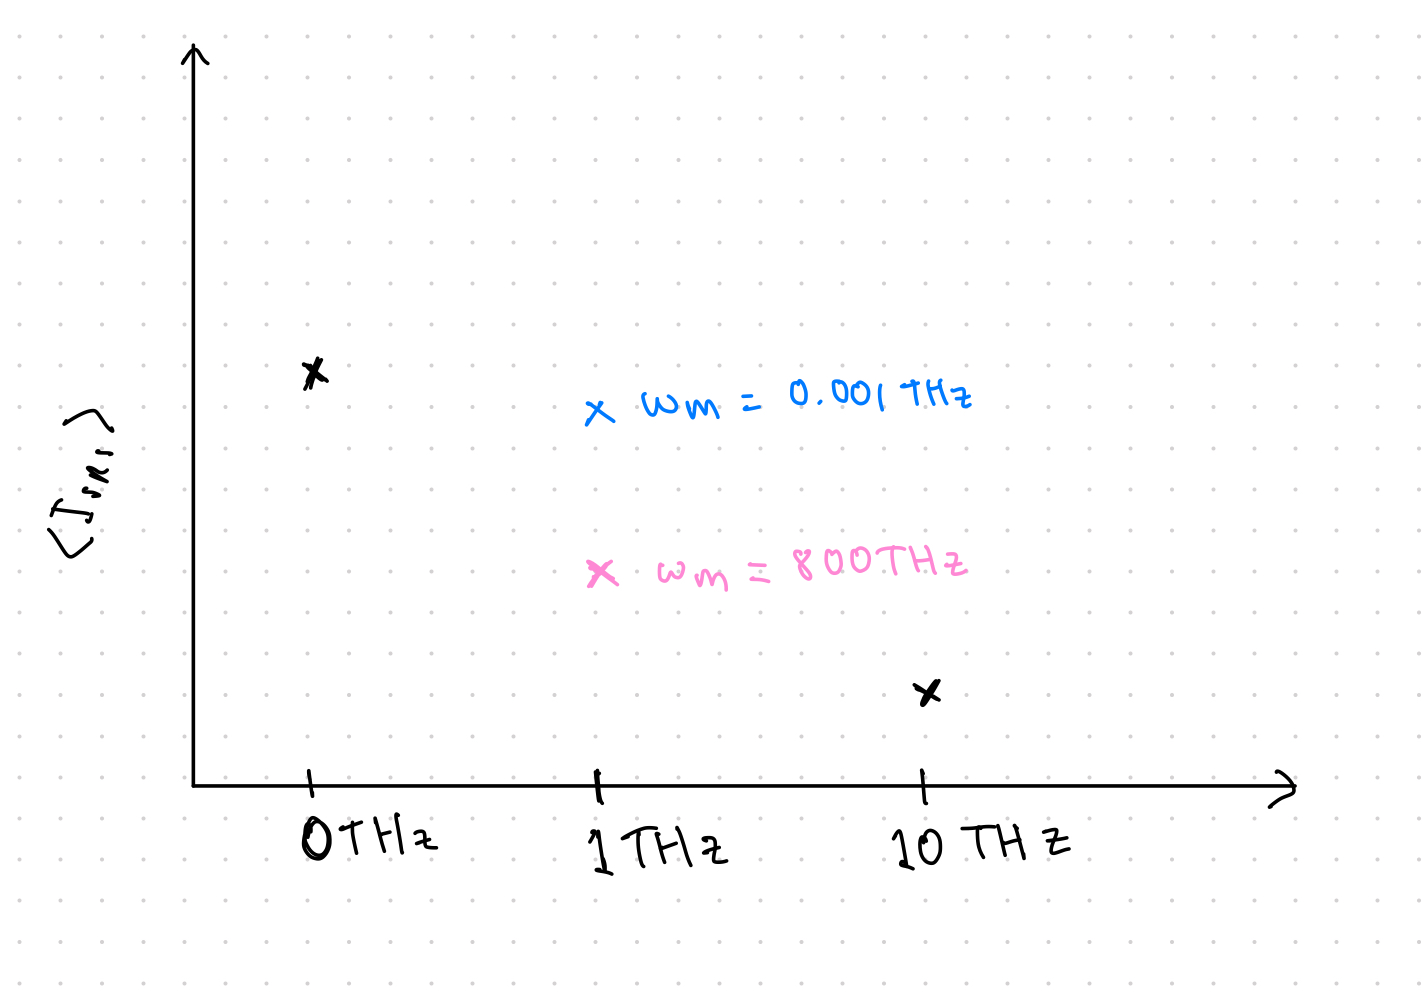
\includegraphics[width=0.75\columnwidth]{Chapters/C5_broadband/ndglass_placeholder.jpeg}
    \caption{placeholder figure for Nd glass sim results}
    \label{fig:NdGlass}
\end{figure}{}

\section{248nm krypton fluoride}\label{sec:248}

\subsection{Base case: $\Delta\omega=0$}

\section{193nm argon fluoride}\label{sec:193}
Excimer lasers have a broad amplification spectrum in the UV when compared to Nd: glass lasers. In this section we consider the argon fluoride (ArF) laser under development at the NRL, which is predicted to have native bandwidth up to 10THz \citep{Obenschain2020}.

\subsection{Base case: $\Delta\omega=0$}

\subsection{Intrinsic bandwidth: $\Delta\omega=5,8,10$ $\si{THz}$}
In this section, we perform a series of simulations at different bandwidths which are considered realistic for ArF laser systems currently under development \citep{Obenschain2020}.

\begin{figure}[ht]
   \centering
    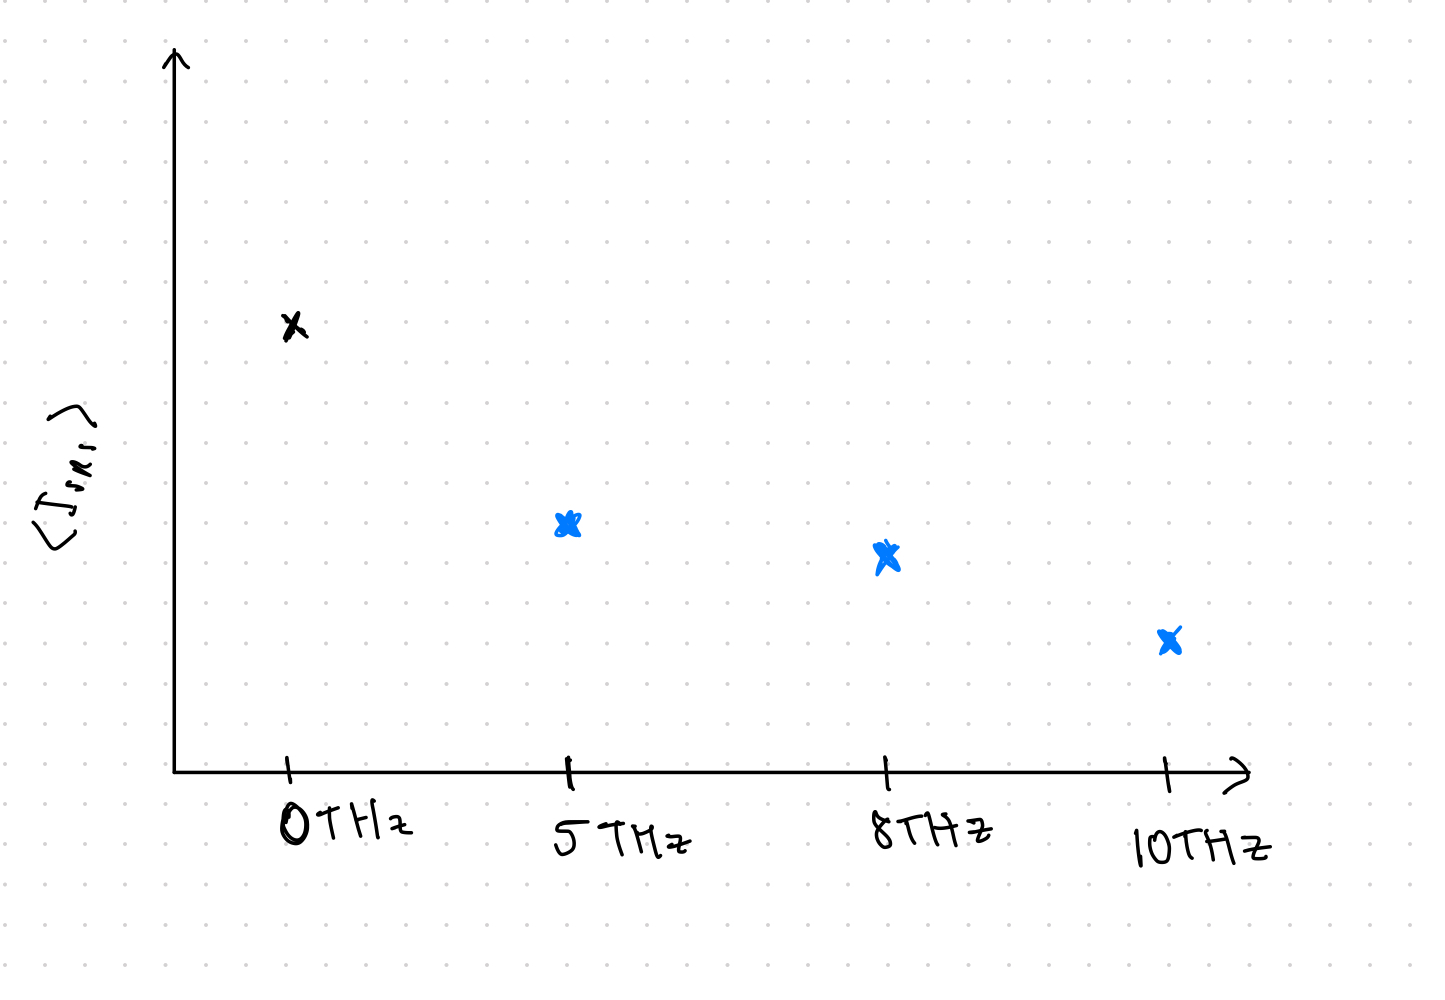
\includegraphics[width=0.75\columnwidth]{Chapters/C5_broadband/arf_placeholder.jpeg}
    \caption{placeholder figure for ArF sim results}
    \label{fig:ArF}
\end{figure}{}


\section{Conclusion}


%\bibliographystyle{plainnat}
%\bibliography{Chapters/C5_broadband/broadband}
